%\documentclass[preprint,floatfix, 11pt] {revtex4} 
\documentclass[11pt,letter]{article}

\newcommand{\rvec}{\mathrm {\mathbf {r}}} 
\usepackage{xcolor}
\usepackage{color, soul}
\usepackage{tabularx}
\usepackage{float}
\usepackage{amsmath}
\usepackage{amssymb}
\usepackage{amsfonts}
\usepackage{mathtools}
\usepackage{bbm}
\usepackage{color}
\usepackage[final]{pdfpages}
\usepackage{bbold}
\usepackage{graphicx}
\usepackage{subfigure}
\usepackage{epsfig}
\usepackage{multirow}
\usepackage{booktabs}
\usepackage{natbib}
\newcommand{\argmin}{\arg\!\min}
\DeclareMathOperator{\Var}{Var}
\DeclareMathOperator{\Cov}{Cov}
\DeclareMathOperator{\E}{\mathbb{E}}
\usepackage{amssymb}
\long\def\/*#1*/{}
\usepackage{setspace}
\usepackage{wrapfig}
\usepackage{ctable}

\usepackage[top=1in, bottom=1in, outer=1in, inner=1in, heightrounded, marginparwidth=1.9in, marginparsep=0.1in]{geometry}

\usepackage{fancyhdr}
\usepackage{lastpage}
\pagestyle{fancy}
\fancyhf{}
\renewcommand{\headrulewidth}{0pt}
\cfoot{ \thepage \hspace{1pt}/\pageref{LastPage}}

\usepackage[utf8]{inputenc}
%\pagenumbering{roman}

\usepackage[USenglish]{babel}
\usepackage{url}


\usepackage{fontspec}
\setmainfont[Ligatures=TeX,
BoldFont=HelveticaNeueMed.ttf]
{HelveticaNeue_Light.ttf}


\newcommand*{\todo}[1]{%
  {\bf \color{red} #1}%
}

\newcommand{\iden}[1]{\mathbb{I}_{#1}}
\newcommand{\bs}[1]{\boldsymbol{#1}}

%\pagestyle{plain}

\begin{document}                                         	

\setstretch{1.1}
%%\begin{center}
%%\textbf{\large Supplemental Materials}
%%\end{center}

\setlength\parindent{0pt}
\setlength{\parskip}{0.7em}

%\pagestyle{empty}
%\begin{center}
{\LARGE \bf %2017 Datathon Report\\
%High-Frequency 
CollegeIndex: A Transparent College Evaluation System 

based on Financial Structure}% with  Soft Power Controlled}
\vspace{2mm}
\\
Yunlin Zhang, Dingzeyu Li, Shanghong Xie, Wodan Ling\\
Team 12
\vspace{-4mm}

%\noindent {\bf Keywords:} 

\section{Topic Overview} 

\begin{figure}[H]
\centering
\vspace{-3mm}
\fbox{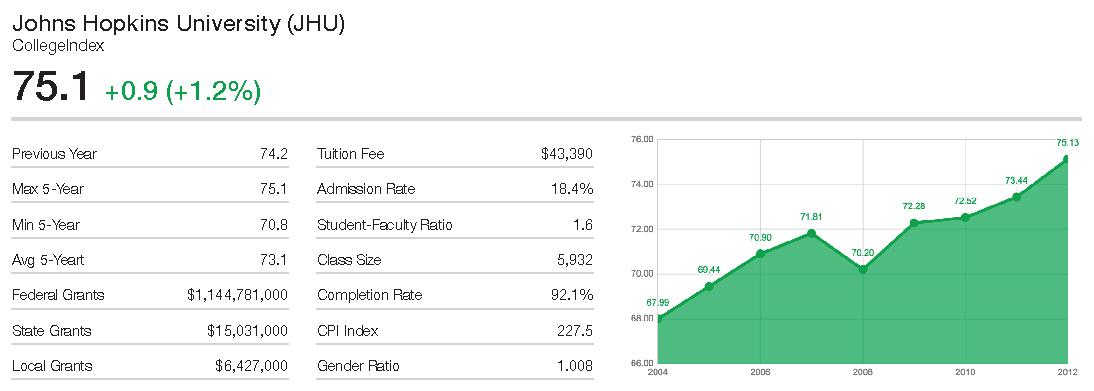
\includegraphics[width=0.99\linewidth]{figure-1.pdf}}
\caption{Index curve of Johns Hopkins from 2004-2012 generate from our proposed evaluation system CollegeIndex. CollegeIndex is a transparent and explainable system, trained on real-world data.
By projecting all the high-dimensional data onto a learned low-dimensional embedding,
we are able to quantify the contribution of each key factors and provide 
 policymakers with customized suggestions for different schools. 
}
\vspace{-3mm}
\label{fig:collegeindex}
\end{figure}

% DONE \todo{Ding, can you update the collegeIndex value for JHU ?:  75.1 (2012),74.2 (2011), max 5-year:75.1, min 5-year: 70.8, ave 5-year:73.1 }

% 1. define topic questions \\
% 2. why it is important
For policymakers at various levels of government, 
it is crucial to determine how to allocate resources to increase appreciation of an institute. 
%While a prospective senior in high school needs to decide where to apply to college to set her path for the rest of her life. 
College ranking score is a way to have a quick understanding of a school's performance. However, existing ranking systems cannot provide an intuitive and quantitative understanding about what kind of financial structure will increase the evaluation.
Evaluation \emph{transparency} is the key to improve the intuitiveness and the decision-making process.
For example, when two colleges receive the same ranking score, the score alone might not tell the 
difference on what areas a school excels at and what are to be improved.

We propose CollegeIndex, a transparent evaluation system trained from a two-stage model composed of Bayesian representation and advanced tree-based learning. Figure \ref{fig:pipeline} shows the pipeline of our CollegeIndex system.  

We are inspired by the stock markets, where financial structure is also a key factor in determining the stock price of a public company. 
% In quarterly financial reports, any non-subtle change in the financial structure would have an impact on the stock value. 
%Financial reports are widely used because 
The structure indicates revenue composition, reveals fiscal robustness, and sheds light on short-term and long-term future plans~\cite{hagenau2013automated,hopkins1996effect,ou1989financial}. 
%However, there is also a large number of metrics to evaluate and compare companies, while there are probably not nearly as many ways that a company is managed. This same line of thinking is applied to analysis of colleges. 
In CollegeIndex, we first extract low dimensional factors from raw financial data using unsupervised learning, then learn the association between the factors and evaluation, and find key features while adjusting for other administration or discipline features. We aim to gain insight into how financial structure of a college and its macroscopic characteristics determine its ranking from external agencies such as U.S. News~\cite{titus2006understanding}.

\begin{figure}[H]
\centering
\includegraphics[width=0.5\linewidth]{pipeline3}
\caption{Schematic for our two-stage CollegeIndex system. } \label{fig:pipeline}
\end{figure}
%By developing a transparent college evaluation system,  
% we aim to provide useful, intuitive, and constructive feedback to students, educators, and government/policymakers, especially on the financial structure of the institute, with administration and discipline features controlled.


%For policymakers at various levels of government and prospective students alike, college ranking is a straightforward way to have a quick understanding of a school's performance. However, existing ranking systems are designed without transparency in mind and details are often not exposed to consumers of this data. For example, when two colleges receive the same ranking score, the score alone might not tell the difference on what areas a school excels at and what are to be improved.

%CollegeIndex is an intuitive metric to visualize and help the decision-making process. In recent years, despite increasing investment in education, higher education of the United States shows a diminishing advantage over its global peers. By analyzing the fundamental financial structure of universities,

Our system, CollegeIndex, has the following distinctive features:
%\vspace{-2mm}

\begin{itemize}
\item
{\bf Intuitive Visualization}. The generated index in the final step is a single value. Very much like the stock market. We can therefore visualize its performance over time. For the general public, this type of visualization is straightforward and conveys the quantitative performance intuitively. Figure~\ref{fig:collegeindex} shows the evaluation generated by our system, CollegeIndex, for Johns Hopkins University. Additionally our feature embedding of financial structure, which will be discussed below, allows us to visualize clusters of institutes, and obtain an intuition understanding of their general characteristics. 

\item {\bf Robust to Missing Data}. 
Our model can work even if the data from colleges is incomplete. This is done using a Bayesian time-dependent generative model. Using this approach has allowed us to work with a dataset of 35750 samples that is missing more than 1 million individual feature values without discarding any samples. 

\item{\bf Explainable Feature Embedding}. 
Our model makes use of representation learning to uncover structures in the financial data of a college and create a set of 5 features from 100 observational features. These new features have very intuitive interpretation and can relay information such as tuition structure (i.e. public colleges have different in-state and out-of-state tuitions while private colleges do not).

\item {\bf Consistent with Existing Metrics}. CollegeIndex is consistent with standard college ranking system. It uses financial structure and basic college characteristics but provides similar results as the standard ranking criteria.  

%\item {\bf Flexible Modeling and Implementation}. When constructing our own CollegeIndex system, we draw inspirations from popular college ranking~\cite{usnews} to mimic a ranking score as the response of the advanced tree-based learning stage. However, the score can be designed arbitrarily and our model can be easily updated to reflect the change. For example, at some point, if policymakers would like to shift the evaluation focus from research outcome to teaching quality, they can easily add new components to this model or reweigh the existing components. The updated index can be computed efficiently.

\end{itemize}

%{\bf{??? Could you explain what do you mean here? @ Ding}}
% I wrote this a long time ago...

% Building a explainable feature embedding for finance-related data has a wider implication beyond the aforementioned advantages. In traditional systems, for example college ranking, is known to be unreliable and can even be gamed with intentional intervention~\cite{dearden2013framing}. the CollegeIndex system complements the existing ones by looking at the raw financial data and providing feedback and suggestions for future improvement. By investigating directly on the financial spendings and earnings, we hope to construct a more fundamental system for evaluating college performance.


\section{Key Findings}
\subsection{Time Series Comparison}

One straightforward way to use the entire CollegeIndex system is to generate a series of evaluations for an institute, based on financial structure, administration, discipline and other features, as shown in Figure 1. Take the visualization one step further. We can plot multiple index curves together, and even overlay with other type of data to gain more insights. Here we show two kinds of visualization enabled by CollegeIndex.
\begin{itemize}
\item Multiple index curves from different colleges. Figure~\ref{fig:curves}(a) shows when we 
compare the MIT, University of Chicago, and University of Notre Dame together, we observe different
rate of progress. While University of Notre Dame exhibits an overall slower pace, MIT only starts to 
fall behind around year 2009. 
\item Generated index with other factors. Looking closely at factors related to the evaluation,  
Figure~\ref{fig:curves}(b) reveals the trend of fine-grained properties, from which more 
detailed analysis could be performed.
\end{itemize}

\begin{figure}[H]
\centering
%\fbox{
\includegraphics[height=1.7in]{multiple_index_curves.png}
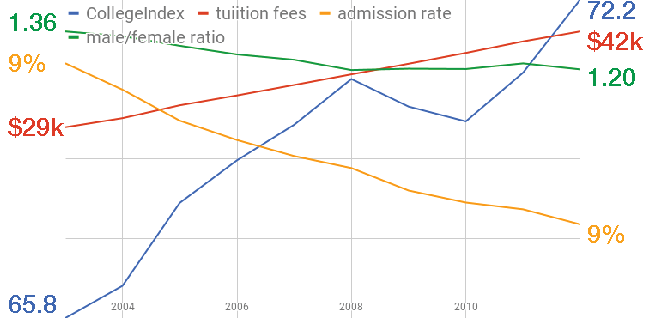
\includegraphics[height=1.7in]{other_data.pdf}
%}
\caption{Left: Overlay of the index curves for University of Chicago (Blue), MIT (Red), and University of Notre Dame from 2003 to 2012. In this multi-curve setting, with a similar starting point, we noticed that UofChicago has progressed much faster than the other peers. Right: Since we would like to explain what contributes to the increase in the evaluation, we can visualize different key factors along with the index. In this example, we observe that the increase of index value, the increase of tuition fees, the decline of admission rate, and the steady drop in gender ratio all occur at the same time.} 
\label{fig:curves}
\end{figure}



\subsection{Clustering}

The first stage of our system reduces 100 features from college financial data down to 5 factors, where we observe an impressive \emph{clustering} learned by our system. 

\noindent Using the lower dimensional embedding of the college financial data, we can perform clustering analysis to deduce if there are any patterns in the financial structure of various types of institutions, and whether this affects their ranking. We used t-distributed stochastic neighbor embedding (t-SNE) for this purpose. The visualization technique only seeks to preserve clusters from the higher dimensional space, but it is clear that the structure discovered from the finances of different types of colleges give them different distributions in this lower dimensional space.


\begin{figure}[H]
\centering
%\fbox{
\includegraphics[width=0.75\linewidth]{public_cluster.png}
%}
\caption{t-SNE visualization of the results of our unsupervised learning on public colleges. From left to right are 4-year, 2-year and under-2-year schools on the same scale. The cluster on the left for 4-year colleges (circled in red) contains 16 of the top 20 public universities ranked by US News which are listed to the left. }
\end{figure}

\subsection{Linear Embedding Factor Loading}

This is the second impressive finding learned from the first stage of the system - every embedding factor can be easily explained. It drastically helps interpretation of the second stage, advanced tree-based model, so helps to interpret the entire system. 

By using a linear mapping from latent embedding to observations, it is very easy for us to visualize the effect that the former has on the latter. This is simply the mapping matrix that we learned in the process. Table \ref{tab:linearloads} summarizes some of the features that were the most sensitive to changes in the embedding in both directions. 
\begin{figure}[H]
\centering
\includegraphics[scale=0.45]{loading.png}
\caption{Factor loading for each of the learned components. Each row represents a different latent dimension while columns are the observations, with darker shades of color representing the two extremes (red = positively associated and blue = negatively associated).  }
\end{figure}

\begin{table}[H]
\begin{tabular}{|c|c|c|c|c|c|}
\hline
Component &  1 &  2 &  3 & 4 & 5\\
\hline
Positive 1 & state grants & avg subsidy & avg subsidy & aid pct & inst grant\\
Positive 2 & total faculty&  operating margin &all employees &  inst grant &  avg subsidy\\
Negative 1 & avg subsidy&  inst grant & tuition 01 &  tuition 05 &  state grant \\
Negative 2 & fed grant pct&  tuition 07 &  inst grant & total faculty& tuition 03 \\
\hline
\end{tabular}
\caption{Linear model loading factors.}\label{tab:linearloads}
\end{table}
Based on these values, we have characterized each component of the embedding and assigned a name to them for reference as follows:
\begin{table}[H]
\begin{tabular}{|p{2cm}|p{4cm}|p{9cm}|}
\hline
Component & Name & Justification\\
\hline
1 & state grant factor& This component has positive sensitivity to state grants but negative sensitivity to federal and institutional grants\\
\hline
2 & public or private tuition structure & This component has positive sensitivity to in district and in state tuition and negative sensitivity to out of state tuitions. However, for private colleges in state and out of state tuitions are the same, so this component reflects the tuition structure difference between public and private colleges\\
\hline
3 & size factor & This component has positive sensitivity to number of employees and expenditures and negative sensitivity to tuitions and grants \\
\hline 
4 & aid factor & This component has positive sensitivity to the aid that students receive and negative sensitivity to tuitions\\
\hline
5 & institution grant factor & This component has positive sensitive to institutional grants and negative sensitivity to state and federal grants.\\
\hline
\end{tabular}
\end{table}
\subsection{Important factors for college ranking}
In the second stage, important features, which contribute to college ranking, are identified separately for public institutes and private institutes (Figure~\ref{fig:publicprivate}). We mimicked methodology of U.S. News~\cite{usnews} to create a standard ranking score. We train on the data to reproduce these scores using our extracted features from financial data and characteristics of the school. The features used in U.S. News calculation are not used in our index calculation process.

%both recreation of US News's ranking score and our system to avoid bias from data leakage.

Financial structure of an institute highly impacts its ranking and the financial structures of public and private institutions are different. Figure \ref{fig:publicprivate} shows the important features, which contribute to college ranking, identified in public institutes and private institutes. Aid factor are important for both public and private institutes. However, there exist different financial characteristics between public institutes and private institutes. State grant factor is important for public institute, whereas it is not identified as informative for private institutes and tuition structure contributes more to private institutes.

In addition to financial structure, student debt is important for ranking in both public and private institutes. Top ranked institutes tend to charge higher tuition fee among both public institute and private non-profit institutes. In terms of the percentage of degrees award in specific majors, engineering impacts both public and private ones, while big difference can be seen in philosophy (impact public institutes) and physical science (impact private institutes). 



\begin{figure}[H]
\vspace{-5mm}
\begin{center}
\includegraphics[scale=0.6]{PublicPrivateGB}
\caption{Comparison of important features for public institutes and private non-profit Institutes}\label{fig:publicprivate}
\end{center}
\vspace{-3mm}
\end{figure}


\vspace{-3mm}
\section{Technical Summary}
\subsection{Exploratory data analysis}

{\bf{Stable Trend}}.  We analyzed financial data for colleges, looking for signs of autoregressive trends in single variate and general trends in multiple variables. We observed that in the case of the vast majority of financial variables, the previous year’s value is a great predictor for this year’s value. This makes sense as colleges have systematic financial planning in place that seek to minimize risk to its operations.
\begin{figure}[H]
\centering
\includegraphics[width=0.70\linewidth]{autoregres}
\caption{Top: all expenditures vs previous period. Bottom: all institutional grants vs previous period. Some variables do not change much from year to year, while others may deviate, but on average the trend for the whole population is to stay the same (on the 45-degree line drawn)}
\end{figure}

However, for public colleges, its operating margin seemed to undergo a regime change in 2002, while revenue and expenditures did not undergo a similar shift, refer to figure \ref{regimeswitch}. Upon further research, we found that there were several accounting guidelines issued by Government Accounting Standards Board (GASB 34, 35, 36) that changed some of the account practices for Government agencies. For our dataset, it only affected public colleges. In order to not confounding our subsequent analysis, only data from academic year 2003 and beyond were used.
\begin{figure}[H]
\centering
\includegraphics[width=\linewidth]{regime_switch.png}
\caption{ Previous year's operating margin vs this year's. Arrow indicates that for public 4-year colleges (left) the data for 2001-2002 lies away from the main population. Private (middle) and for profile (right) schools do not show this behavior.}\label{regimeswitch}
\end{figure}

\begin{figure}[H]
\centering
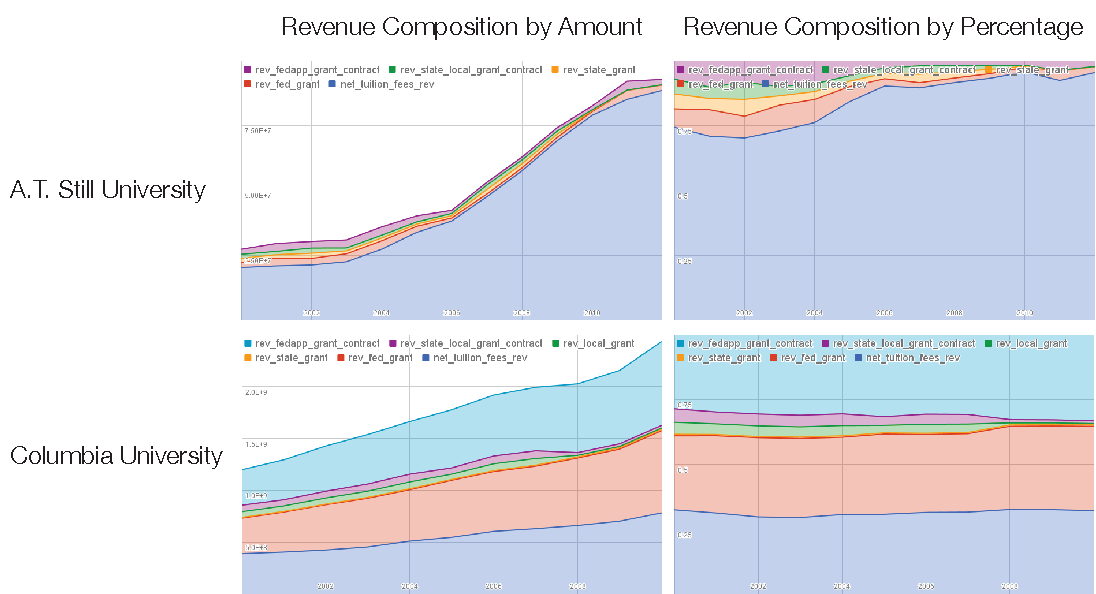
\includegraphics[width=\linewidth]{data-explore.pdf}
\caption{Revenue composition for two colleges, A.T. Still University and Columbia University. On the left is  the composition by amount. We can see that for both universities, the overall revenue is increasing. On the right is the composition by percentage. 
We observe that the proportion of tuition fees for A.T. Still University has grown significantly, whereas Columbia University maintains a relatively stable structure. 
}
\label{fig:data_explore}
\end{figure}

\paragraph{Revenue Proportion Analysis} We hypothesize that different universities would have different financial structures. One easy way to explore is to investigate revenue sources and proportions. Figure~\ref{fig:data_explore} shows our initial data exploration in two universities with a variety of 
 different properties including sizes, focuses, geographical locations, etc.


\subsection{Data Engineering and Manipulation}
\paragraph{College Financial.}
Based on our exploratory analysis, since many variables show highly autoregressive trends, we decided to forward fill the missing values for the columns with the highest autocorrelations. All other missing values are kept and inferred as part of variational inference in our Bayesian model. In addition, since the data has time dependence, we added additional columns that contain the percentage change for that variable from the previous period. With the addition of the new features, we ended up with a total of 100 features. 

\paragraph{Table Merging.} We need to relate two tables, college and college\_financials. 
Unfortunately the names of the university do not match 100\% -- some differ only by simple hyphens, some other differences are more difficult to handle. We leverage a multi-level fuzzy match approach. First, we extract the unique university names in both datasets to reduce the computation complexity. Second, for each name in colleges.csv, we look for a match in college\_financial.csv. We filter out most of the universities by comparing state, city, and zipcode. Once we have a pool of candidates, we perform a fuzzy text string matching algorithm on the names and choose the one with highest similarity score. Last, we merge the two tables based on the robust multi-level fuzzy-matched names. 
%During this matching process, we are able to merge more than 85\% of the universities in the tables.



\subsection{Model}
\paragraph{Time dependent representation learning} The first stage of our model is a generative model that tries to find a lower dimensional embedding for the financial structure of a particular school. This is inspired by recent advancements in manifold learning, in which the conjecture is that high dimensional data is in fact generated by some mapping function from a low dimensional manifold. A special case of this is when the manifold and mapping functions are both linear, and this is the venerable principal component analysis. The nonlinear analogue is known as the autoencoder, in which the mapping function is a neural network. Due to the large amount of missing data and time dependence in the data, we formulated Bayesian generative versions of these models and performed inference by marginalizing out the missing data.

We posit that there exists some latent space with dimension $d$ from which our observed data in dimension $k$ is generated. For our system, $k=100$ and $d=5$ The natural interpretation is that there are only so many interest aspects of the entity generating the data, where all observations are based on these aspects. A geometric example is a helix. It is a three-dimensional object, but you can fully specify where you are using a single number. In machine learning literature this is referred to as representation learning. We shall reference to the particular values inferred for each data point as its embedding.

Since there is time dependence in the data, we further posit that there is some innovation applied to the hidden states at each time period. This method takes inspiration from stochastic volatility modeling of time series~\cite{rwbnn}. We apply a Gaussian innovation to the latent embeddings at each time step for simplicity. A linear transformation could also be applied, though due to the brevity of the time period considered (2003-2012), and the high degree of autocorrelation observed in the data, we decided to ignore it for this work. 

To address the issue of missing data, we looked to Bayesian approaches for imputing data, where the methodology makes no distinction between parameters of the model and missing data: they have a joint posterior distribution, conditional on observed data~\cite{bda3}. The model is by definition probabilistic, and we can marginalize out all the different possible values for the missing values over their respective probabilities. 

Please refer to Appendix \ref{model} for our model specification. Inference and learning are carried out using variational inference. 

\begin{figure}
\centering
\includegraphics[scale=0.6]{model_diag}
\caption{Bayesian network representation of the conditional dependences in our model. At each time step, an entity is in a probabilistic state $H_i$, and from it produces an observation $X_i$}
\end{figure}


\paragraph{Advanced tree-based learning}
In the second stage, we incorporate the lower dimensional embeddings for the financial structure extracted from the first stage, and other characteristics of university to identify important features which contribute the most to college ranking. Random forest with conditional inference tree and gradient boosting with regression tree \cite{friedman2001elements} are implemented to analyze public institute and private non-profit institute separately.          



\subsection{Detailed Analysis}
%\paragraph{Tree-based Model}
\subsubsection{Tree-based Models}
Since U.S.News ~\cite{usnews} does not provide exact ranking scores, we draw inspirations from it to mimic a standard ranking score as the response of the advanced tree-based learning stage. The standard ranking score is a weighted score (weights are similar to the ones used by U.S.News) of completion rate, faculty average salary, student-faculty ratio, class size, acceptance rate, SAT score and education expenditure per student. 

The low-dimensional embeddings extracted from the time-dependent generative model with linear function or deep neural network are treated as additional features which contribute to college ranking. The other features considered are institution type, tuition fee, loan debt, state of the institute, and percentage of degree awarded in several majors.

The performance of tree-based methods using financial embeddings from linear version and deep neural network version is similar. We randomly selected two third of data as training set and the remaining one third as test set. Table \ref{tab:MSElinear} and \ref{tab:MSENN} summarize the prediction performance. The results show that the prediction performance of using linear version embeddings and neural network embeddings are similar and using linear version embeddings results in more stable prediction. Thus, we omit the results of using neural network embeddings on full data to be concise. Besides, gradient boosting performs better than random forest in terms of prediction and stability.


\subparagraph*{Public Institute}
The results of random forest and gradient boosting are similar (Figure \ref{fig:crf_public} and Figure \ref{fig:gb_public}).
The common features among top 10 important features identified for public institute in the two methods are state grant factor, aid factor, out-of-state tuition fee, number of students in the cumulative loan debt cohort, cumulative loan debt at the 25th percentile, and the percentage of degrees awarded in engineering, foreign languages, and philosophy.

\begin{figure}[H]
%\centering
\begin{center}
\includegraphics[scale=0.4]{crf_public}
\caption{Important features for Public Institute through Random Forest}\label{fig:crf_public}
\vspace{-3mm}
\begin{flushleft}\small 
\centering
index 1: state grant factor; index 2: tuition structure factor; index 4: aid factor.
\end{flushleft}
\end{center}
\end{figure}

\begin{figure}[H]
\begin{center}
\includegraphics[scale=0.4]{gb_public}
\caption{Important features for Public Institute through Gradient Boosting}\label{fig:gb_public}
\vspace{-3mm}
\begin{flushleft}\small 
\centering
index 1: state grant factor; index 2: tuition structure factor; index 4: aid factor.
\end{flushleft}
\end{center}
\end{figure}


\subparagraph{Private Non-profit Institute}
Figure \ref{fig:crf_private} and Figure \ref{fig:gb_private} show the important features for private non-profit institute identified by random forest and gradient boosting, respectively. The feature that impacts university ranking the most is the tuition fee. Aid factor (6.5\%) is identified as important as the same for public institutes and public or private tuition structure contributes about 6\% (according to gradient boosting) for private institutes. The number of students who have cumulative loan debt at the 25th percentile is again identified as top 10 informative features. The majors which impact university ranking are physical science, engineering, and area/ethnic/cultural studies.

\begin{figure}[H]
\begin{center}
\includegraphics[scale=0.4]{crf_private1}
\caption{Important features for Private Non-profit Institute through Random Forest}\label{fig:crf_private}
\vspace{-3mm}
\begin{flushleft}\small 
\centering
index 1: state grant factor; index 2: tuition structure factor; index 4: aid factor.
\end{flushleft}
\end{center}
\end{figure}


\begin{figure}[H]
\begin{center}
\includegraphics[scale=0.4]{gb_private1}
\caption{Important features for Private Non-profit Institute through Gradient Boosting}\label{fig:gb_private}
\vspace{-3mm}
\begin{flushleft}\small 
\centering
index 1: state grant factor; index 2: tuition structure factor; index 4: aid factor.
\end{flushleft}
\end{center}
\end{figure}

\subsubsection{Linear vs Neural Network Embedding Learning}
We attempt to use both linear and nonlinear mapping from the latent space to observation space, with the latter using neural networks. As shown in the above analysis, performance of the linearly and nonlinearly extracted features are similar, the latter giving a larger variance. Refer to Figure~\ref{fig:elbo}. the loss function (evidence lower bound or ELBO) from the optimization. 

\begin{figure}[H]
\centering
\includegraphics[width=\linewidth]{elbo.png}
\caption{ELBO for linear (left), neural network ReLU activation (middle) and neural network with tanh activations (right) for the mapping from latent space to observation space.}\label{fig:elbo}
\end{figure}

With the wrong activation function for the neural network, the trained network can have a large variance (as in the case of ReLU activation). Thought this seems to be ameliorated by using the tanh activation, it does not improve performance in the subsequent step. Therefore we concluded that for this particular application, a linear function is sufficient. 

\section{Conclusion and Discussion}
We have demonstrate a pipeline to condense financial information and combine it with other features into a numerical metric that can be used to evaluation and rank colleges, and we've named the system CollegeIndex. Using this system, someone can gain transparency to the contributing factors behind the score, and a numerical value that can be used to rank colleges resembling how popular services such US News has been doing so. 

These methodology can be further expanded and applied to the capital market. Traditionally analysis has been based on hand engineered features. By applying our first stage, Bayesian representation learning, we are able to uncover structures and patterns in how companies operates and reason about over and under-performance with respect to a company's peer. 

On the more technical side, though the neural network approach did not show better performance than a linear model, it can still be applied to other problems where a linear model would fail. For example, noisy sequence of images. However, a caveat for adopting this approach is the drastically increased run time from running a Bayesian inference in addition to training a potentially deep neural network. 

Through the data analysis and exploration, we also found race and gender can be chosen as a contributing factor to the score of an institute. However, these findings just reaffirms existing biases in the world, and if they were incorporated into the analysis it can perpetuate these biases. Just because a high ranking college has more white or male students, does not mean a school should recruit more white male students to boost its rankings. Therefore we excluded them from our analysis. We do, however, recognize their value in socially responsible machine learning.


% Additional information (e.g. roadblocks encountered, caveats, future research areas, and unsuccessful analysis pathways) may be placed in an appendix (does not count towards the length limits specified above).


\appendix
\renewcommand\thetable{\thesection\arabic{table}}

\setcounter{table}{0}
\setcounter{table}{0}
\renewcommand{\thetable}{A\arabic{table}}


%\renewcommand\thefigure{\thesection\arabic{figure}}

%\setcounter{figure}{0}
%\setcounter{figure}{0}
%\renewcommand{\thetable}{A\arabic{figure}}

\section{Prediction Performance}

\begin{table}[H]
\centering
\begin{tabular}{|l|l|l|}
         \hline                                                 & Mean RMSE\footnotemark[1] & SD RMSE   \\
         \hline 
Gradient Boosting - Public Institute                              & 0.0196    & 6.3939e-04 \\
Gradient Boosting - Private Institute                             & 0.0295    & 9.7297e-04 \\
\hline
Random Forest with Conditional Inference Tree - Public Institute  & 0.0630    & 2.2749e-03 \\
Random Forest with Conditional Inference Tree - Private Institute & 0.0752    & 1.5632e-03 \\
\hline
\end{tabular}
\caption{Prediction performance of using Financial Features Learned from Linear Generative Model}\label{tab:MSElinear}
\begin{flushleft}\small\footnotemark[1]RMSE: root mean-squared-error.
\end{flushleft}
\end{table}

\begin{table}[H]
\centering
\begin{tabular}{|l|l|l|}
              \hline                                                    & Mean RMSE\footnotemark[1] & SD RMSE    \\
              \hline
Gradient Boosting - Public Institute                              & 0.0205          & 7.2540e-04
 \\
Gradient Boosting - Private Institute                             & 0.0292           & 1.0448e-03\\
\hline
Random Forest with Conditional Inference Tree - Public Institute  & 0.0653            & 2.2836e-03
 \\
Random Forest with Conditional Inference Tree - Private Institute &0.0750           & 1.8032e-03 \\
\hline
\end{tabular}
\caption{Prediction performance of using Financial Features Learned from Generative Model via Neural Network} \label{tab:MSENN}
\begin{flushleft}\small\footnotemark[1]RMSE: root mean-squared-error.
\end{flushleft}
\end{table}


\section{Visualization}
\subsection{Clustering for all college sectors}
\begin{figure}[H]
\centering
\includegraphics[width=0.5\linewidth]{tsne_linear_all.pdf}
\caption{t-SNE clustering plot separated by sector. The columns are public, private and for-profit college, and the rows are 4 year, 2 year and less than 2 year colleges. The scales are the same for all plots. }
\end{figure}
\section{Model specification}
\subsection{Generative state space model}\label{model}
We used the follow formulation for the condition probabilities
\begin{align*}
H_1 & \sim \mathcal{N}(0, \iden d )\\
\epsilon_i &\sim \mathcal{N}(0, 0.1 \iden d ) & i=2,...,T\\
H_i & \sim H_{i-1} + \epsilon_i\\
X_i & \sim \mathcal{N}(f(H_i;\theta_1,...,\theta_M), \iden k )
\end{align*}
Here $f:\mathbb{R}^d\rightarrow\mathbb{R}^k$ is the mapping from latent embeddings to observations, and it parametrized by the $\theta$ variables. For the linear model, we have the following forms for $\theta$ and $f$
\begin{align*}
\theta &\in \mathbb{R}^{d\times k}\\
\theta_{i,j} &\sim \mathcal{N}(0,1)\\
f(H;\theta) &= H\theta 
\end{align*}
And for the neural network we have
\begin{align*}
\theta ^ {(i)} &\in \mathbb{R} ^ {p_{i-1}\times p_i}\\
\theta ^ {(i)}_{jk} &\sim \mathcal(0,1)\\
f(H;\theta) &= g(g(g(H\theta^{(1)})\theta^{(2)})\theta^{(3)})
\end{align*}
Where $g$ is the neural network activation function (we tried ReLU and tanh)

\bibliographystyle{plain}
\bibliography{ref}



\end{document}
